% Chapter 2

\chapter{Marco Teórico} % Main chapter title

\label{Chapter2} 

El objetivo de este capítulo fue revisar los fundamentos de la teoría de los sistemas de comunicaciones móviles, comenzando con los diferentes modelos de despliegue para BS y UE, se estudió las características de una geometría estocástica y se repasó la teoría del concepto celular, es decir, la geometría celular clásica que sirve para la eficiencia en la planificación de los recursos y por lo tanto el problema más importante en estos sistemas: los efectos de la interferencia.\newline

Después se ahondó en las pérdidas en un sistema celular por medio de los modelos de canal más comunes y con su caracterización en parámetros a larga y pequeña escala, p.ej., la pérdida por trayectoria y el desvanecimiento de las señales de radio. Además, se revisaron los diferentes esquemas de acceso al medio en comunicaciones móviles.\newline

Finalmente, se revisaron los aspectos de la teoría del tráfico en telecomunicaciones, los organismos más importantes de estandarización de redes móviles y algunos conceptos de las simulaciones a nivel de sistema orientados a eventos discretos en conjunto con los lenguajes de programación más utilizados.\newline


%----------------------------------------------------------------------------------------
%	SECTION 
%----------------------------------------------------------------------------------------

\section{MODELADO DEL DESPLIEGUE CELULAR}

La teoría del diseño celular da una forma simplificada de un diseño idealizado para redes móviles, esta se desarrolló en la literatura desde el comienzo del concepto celular [1975 aprox.], sin embargo este despliegue uniforme que propone la teoría celular, es poco realista ya que nunca se tiene una instalación regular, esto debido a que la densidad del tráfico varia espacial y temporalmente. En el despliegue de BS, frecuentemente en ubicaciones donde se concentraba mayor cantidad de tráfico lo que se realiza es instalar otra BS y por lo tanto esto rompe con esta uniformidad.\newline

En el modelado de posicionamiento de las estaciones base y los usuarios existen diferentes estrategias de despliegue (como se puede ver en la \textit{Figura~\ref{fig:BSs}}):

\begin{figure}[th]
\centering
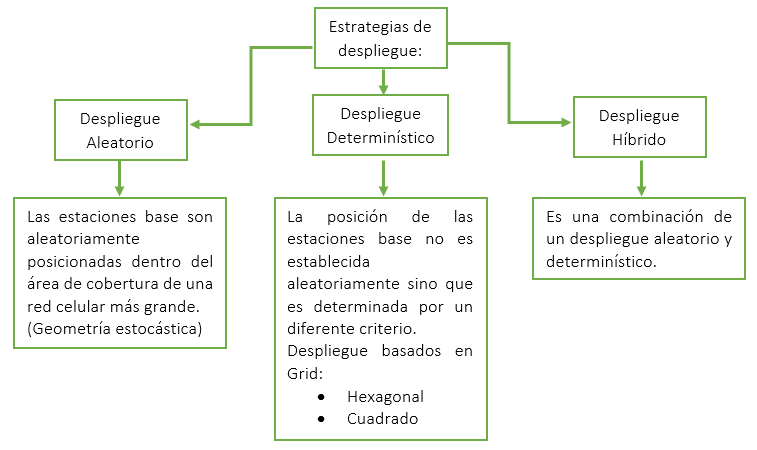
\includegraphics[scale=1]{Diferentes estrategias de despliegue para BSs}
\decoRule
\caption[Diferentes estrategias de despliegue para BSs]{Diferentes estrategias de despliegue para BSs}
\label{fig:BSs}
\end{figure}

\subsection{Procesos puntuales (PP)}
\textit{Point Process} \parencite{Haenggi2009}\newline

En primer lugar, para un despliegue aleatorio, la base son los procesos puntuales ya que son los objetos elementales estudiados en la teoría de geometría estocástica.\newline

Visualmente, un proceso puntual se puede representar como una colección aleatoria de puntos en el espacio. Más formalmente, un proceso puntual (PP) es un mapeo medible $\Phi$ desde algún espacio de probabilidad al espacio de medidas puntuales (una medida puntual es una medida que es localmente finita y que solo toma valores enteros) en algún espacio $E$.\newline

Algunas dicotomías sobre procesos puntuales en el espacio Euclidiano $\mathbb{R}^{d}$ son las siguientes:\newline

\begin{itemize}
    \item Un PP puede ser simple o no. Es simple si la multiplicidad de un punto es como máximo uno (no hay dos puntos en la misma ubicación).
    \item Un PP puede ser estacionario o no. La estacionariedad se cumple si la ley del proceso puntual es invariante por traslación.
    \item Un PP puede ser Poisson o no. En la siguiente subsección se proporciona una definición formal de los procesos puntuales de Poisson (PPP).
\end{itemize}

Antes de entrar a la teoría de los PPP, es necesario definir un Proceso de Poisson.

\subsection{Procesos de Poisson}

Los procesos de Poisson son altamente utilizados para representar o modelar fenómenos en las telecomunicaciones, p. ej. la generación de llamadas telefónicas.\newline

Algunas propiedades de los procesos de Poisson son las siguientes \parencite{ PoissonMedium}:

\begin{itemize}
    \item Se compone de una secuencia de variables aleatorias $X1, X2, X3, ... Xk$, de modo que cada variable representa el número de ocurrencias de algún evento, durante un intervalo de tiempo.
    \item Es un proceso estocástico. Cada vez que ejecuta el proceso de Poisson, producirá una secuencia de resultados aleatorios diferentes según alguna distribución de probabilidad.
    \item Es un proceso discreto. Los resultados del proceso de Poisson son el número de ocurrencias de algún evento en el período de tiempo especificado, que sin duda es un número entero, es decir, un número discreto.
    \item Tiene incrementos independientes. Lo que esto significa es que el número de eventos que el proceso predice que ocurrirá en cualquier intervalo dado, es independiente del número en cualquier otro intervalo disjunto.
    \item Las variables constitutivas del proceso de Poisson $X1, X2, X3, ... Xk$ tienen una distribución idéntica.
    \item Las variables constitutivas del proceso de Poisson $X1, X2, X3, ... Xk$ tienen una distribución de Poisson , que viene dada por la Función Masa de Probabilidad (PMF):
\end{itemize}

\begin{equation}
    P_{X}(k)=\frac{e^{-\lambda}*\lambda ^{k}}{k!}
    \label{eqn:Poisson}
\end{equation}

La fórmula anterior nos da la probabilidad de ocurrencia de $k$ eventos en unidad de tiempo, dado que la tasa de ocurrencia promedio es $\lambda$ eventos por unidad de tiempo.\newline

Los procesos de Poisson tienen una subestructura notable. Aunque el número de eventos ocurridos se modela usando una distribución de Poisson discreta, el intervalo de tiempo entre eventos consecutivos se puede modelar usando una distribución exponencial, que en contra, es una distribución continua \parencite{PoissonMedium}.\newline

\subsection{Procesos Puntuales de Poisson (PPP)}\label{PPP_C4}
\textit{Poisson Point Process} \parencite{Haenggi2009}\newline

Ahora bien, sea $\gamma$ una medida localmente finita en algún espacio métrico $E$. Un proceso puntual $\Phi $ es Poisson en $E$ si:

\begin{itemize}
    \item Para todos los subconjuntos disjuntos $A1, ..., An$ de $E$, las variables aleatorias $\Phi(Ai)$ son independientes.
    \item Para todos los conjuntos $A$ de $E$, las variables aleatorias $\Phi(A)$ son Poisson.
\end{itemize}

Una propiedad clave establece que condicionalmente $\Phi(A)= n$, estos $n$ puntos están ubicados independientemente (y de manera uniforme para un PPP homogéneo) en $A$.\newline

\begin{itemize}
    \item Un PPP puede ser homogéneo o no. En el caso homogéneo, la densidad de los puntos es constante en el espacio (también conocidos como HPPP).
    \item El PPP homogéneo es estacionario y simple. Esto puede considerarse como el proceso puntual más simple (y más natural).
\end{itemize}

Un PPP ofrece un práctico marco computacional para diferentes cantidades de red de interés. El marco para las PPP no homogéneas también está bien desarrollado, aunque es más técnico que el del caso homogéneo. Se pueden usar para modelar distribuciones de usuarios que no son uniformes en el espacio.\newline

%	SUB-SECTION 
%----------------------------------------------------------------------------------------

\subsection{Geometría Clásica Celular}

Ahora bien, para un despliegue determinístico, se suele optar por un esquema hexágonal el cual recurre a la teoria clasica celular donde se busca que los sistemas celulares brinden una determinada cobertura para un servicio, dividiendo el área geográfica en segmentos llamados celdas donde el espectro de frecuencia también es dividido en canales y estos son agrupados para repartirse entre las celdas. Estos sistemas logran una alta capacidad gracias al reúso del canal de comunicación permitiendo a las estaciones base compartir los canales, sin embargo, este reúso da como resultado una interferencia co-canal generada solamente entre usuarios que comparten el mismo canal, lo cual limita el rendimiento y capacidad de un sistema celular dado que los efectos de esta interferencia son altamente dependientes con los aspectos del sistema \parencite{Tranter2003} como lo son el tipo de acceso múltiple del sistema, el número de usuarios compartiendo el canal, el canal de propagación, la perdida por trayectoria, el desvanecimiento, entre otros.\newline

Los sistemas celulares son caracterizados por \parencite{Correia2018}:
\begin{itemize}
    \item Ser limitados por la interferencia (capacidad).
    \item Servir a una alta densidad de usuarios.
    \item Considerar la disponibilidad del espectro solo como un factor limitante.
    \item Reúso de frecuencias.
    \item Uso de Estaciones Base de baja potencia.
    \item Tener celdas de distintas coberturas.
    \item Permitir \textit{handover}.
\end{itemize}

\subsection{Planeación Celular}

Una buena planeación celular es de crucial importancia para lograr un buen rendimiento del sistema y la provisión de una buena Calidad de servicio (QoS).\newline

La planeación celular consiste en:
\begin{itemize}
    \item Colocación de BSs y establecimiento de coberturas
    \item Optima administración de recursos de radio.
    \item Minimización de interferencia.
\end{itemize}
La planeación celular se desempeña de acuerdo a:
\begin{itemize}
    \item Morfología del área de servicio y modelos de propagación.
    \item Perfiles de usuario y modelos de tráfico.
\end{itemize}
Considerando:
\[R\to Radio\ de\ cobertura\ de\ la\ celda\] 
\[D_r\to Distancia\ de\ reuso\ de\ celda\ co\_canal\] 
\[d_u\to Distancia\ unitaria\ entre\ los\ centros\ de\ dos\ celdas\ adjacentes\] 
\[d_u=\sqrt{3}R\] 
\[Llegando\ a\ una\ distancia\ de\ reuso\ normalizada\ D_n\] 
\begin{equation}
D_n=i^2+ij+j^2, donde: i!=0, j!=0
\label{eqn:DistReuso}
\end{equation}
\begin{equation}
=>\ D_r=D_nd_u
\label{eqn:Dn}
\end{equation}
\[\textrm{á}rea\ de\ una\ celda\ S_{cel}\] 
\begin{equation}
S_{cel}=(3\sqrt{3}/2)R^2
\label{eqn:S}
\end{equation}
\[\textrm{á}rea\ de\ un\ cluster\ S_{clu}\] 
\begin{equation}
S_{clu}=(3\sqrt{3}/2)D^2_nd^2_u
\label{eqn:Sclus}
\end{equation}
\[Número\ de\ celdas\ por\ cluster,\ N_{cc}\ \textrm{ó}\ tambi\textrm{é}n\ conocido\ como\ ``factor\ de\ reuso''\ \] 
\begin{equation}
N_{cc}=\frac{S_{clu}}{S_{cel}}
\label{eqn:N}
\end{equation}

$Siendo\ valores\ posibles\ para\ N_{cc}\ ,\ \ \ \ 1,\ 3,\ 4,\ 7,\ 9,\ 12,\ 13,\ .\ .\ .\ $\textit{[Véase Figura~\ref{fig:clusterizacion} y Figura~\ref{fig:celdascocanal}]}.\newline

Para implementar el reúso, se deben asignar un conjunto de canales disponibles para un grupo de celdas, el clúster y repetir ese conjunto a través de toda el área de servicio.

\begin{figure}[th]
    \centering
    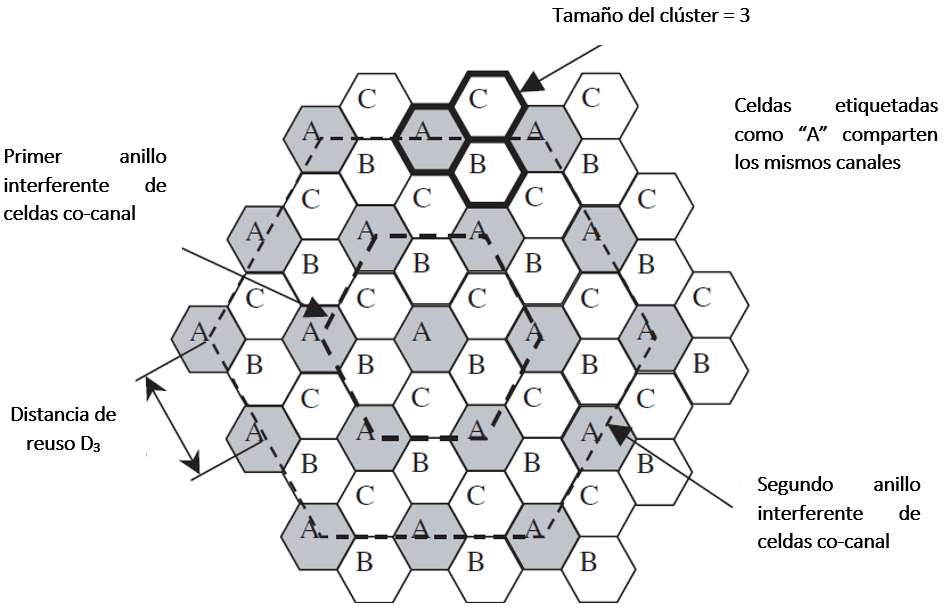
\includegraphics[scale=.5]{Figures/Clusterización de celdas con un factor de reúso de 3 celdas}
    \decoRule
    \caption[Clusterización de celdas con un factor de reúso de 3 celdas]{Clusterización de celdas con un factor de reúso de 3 celdas, [Fuente: Tranter 2003]}
    \label{fig:clusterizacion}
\end{figure}
\begin{equation}
N_{ch/c}=\frac{N_{ch/s}}{N_{cc}} 
\label{eqn:Nch}
\end{equation}
\[N_{ch/c}\to Numero\ de\ canales\ por\ celda\] 
\[N_{ch/s}\to \ Numero\ de\ canales\ en\ el\ sistema\] 
\[N_{cc}\to Numero\ de\ celdas\ por\ cluster\ \] 
La relación de reutilización co-canal,$\ r_{cc}\ $es usada para caracterizar clústeres\
\begin{equation}
r_{cc}=\frac{D_r}{R}=\sqrt{3N_{cc}}
\label{eqn:}
\end{equation}
Un valor grande de $r_{cc}$ corresponde a:
\begin{enumerate}
\item  Una baja interferencia co-canal
\item  Baja capacidad del sistema
\end{enumerate}
El clúster es escogido lo más pequeño posible tomando los umbrales de interferencia en consideración \parencite{Correia2018}.
\[GSM,\ {N}_{cc}=4\] 
\[UMTS,\ {N}_{cc}=1\] 
\[LTE,\ {N}_{cc}=3\] 
\begin{figure}[th]
\centering
\includegraphics[scale=.6]{Figures/Localización de celdas co-canal con distintos factores de reuso}
\decoRule
\caption[Localización de celdas co-canal con distintos factores de reúso]{Localización de celdas co-canal con distintos factores de reúso, [Fuente: Tranter 2003]}
\label{fig:celdascocanal}
\end{figure}
Diferentes tamaños de celda son usadas para distribuciones no uniformes de tráfico \parencite{TurjmanSmallCells}.\newline
\begin{figure}[th]
\centering
\includegraphics[scale=.5]{Figures/Sistema celular con celdas de tamaño no uniforme}
\decoRule
\caption[Sistema celular con celdas de tamaño no uniforme]{Sistema celular con celdas de tamaño no uniforme, [Fuente: Yacoub 1993]}
\label{fig:nouniformcells}
\end{figure}

El uso de diferentes tamaños de celdas:\newline
•	Conduce a un incremento de interferencia, debido a la poca uniformidad en la estructura celular.\newline
•	Requiere cuidado adicional en el despliegue de BSs

\subsection{Planeación de frecuencia}
La decisión de bandas de frecuencia para ser usadas en los diversos sistemas de comunicaciones es decidida por la ITU. La asignación de canales en una banda dada para un operador es decidido a nivel nacional por un cuerpo regulatorio, IFT en México. El hecho de que el espectro es muy escaso incita a un eficiente uso de frecuencias.\newline

El número de frecuencias (portadoras, canales de radio) por celda $N_{fc}$ depende del clúster, $N_{cc}$, y del número de frecuencias en el sistema $N_{fs}$
\begin{equation}
    N_{fc}={N_{fs}}/{N_{cc}}
    \label{eqn:Nfc}
\end{equation}

Debido a la limitación en el número de frecuencias, debe haber una compensación entre la interferencia $N_{cc}\ $y la capacidad$\ N_{ch/c}\ $en el sistema.\newline

La asignación de frecuencias de las celdas debería reducir la interferencia de celda-adyacente maximizando la separación de las frecuencias en una celda.\newline

En un simple sistema celular, las frecuencias deberían ser asignadas a las celdas de acuerdo a:\newline
\begin{equation}
    f_{ij}=i+N_{cc}\ (j-1)
    \label{eqn:fij}
\end{equation}

\[i=1,\ \dots ,\ N_{cc}\] 
\[j=1,\ \dots ,\ N_{fc}\] 

Cuando $N_{sc}$ sectores por celdas son implementados, cada sector deberá contener su propio grupo de frecuencias:\newline
\begin{equation}
    f_{ijk}=i+N_{cc}\ \left(k-1\right)+N_{cc}\ N_{sc}\ (j-1)
    \label{eqn:fijk}
\end{equation}

\[i=1,\ \dots ,\ N_{cc}\] 
\[j=1,\ \dots ,\ N_{fc}\] 
\[k=1,\ \dots ,\ N_{sc}\] \\


%	SUB-SECTION 
%----------------------------------------------------------------------------------------

\subsection{Interferencia en los sistemas de comunicaciones}

En general el receptor recibe:\newline
\begin{equation}
\mathrm{SNIR=}\frac{S}{I+N}
\label{eqn:SNIR}
\end{equation}

Donde:
\[S\to Potencia\ de\ portadora\ de\ la\ se\textrm{\~{n}}al\ deseada\] 
\[I\to Potencia\ de\ las\ portadoras\ de\ las\ se\textrm{\~{n}}alees\ interferentes\] 
\[N\to Potencia\ del\ ruido\] 

Los sistemas de comunicaciones móviles se caracterizan por ser sistemas limitados por interferencia, donde I domina sobre N, por lo tanto la participación del ruido N puede ser ignorada \parencite{Correia2018}.\newline

Quedando entonces como la relación portadora a interferencia:\newline
\begin{equation}
\frac{S}{I+N}\ \ \cong \ \ \frac{S}{I}\ \ \to \ \ SIR
\label{eqn:SIR}
\end{equation}

La interferencia co-canal $I_{cc}$ es un problema aceptado en los sistemas de comunicaciones móviles. \newline

La estimación de la relación portadora a interferencia co-canal ${S}/{I_{cc}}$es calculada de acuerdo  a las siguientes asunciones:

\begin{enumerate}
\item  Todas las celdas son del mismo tamaño
\item  La potencia radiada por todas las BSs son iguales
\item  Todas las BSs tienen antenas omnidireccionales
\item  El decaimiento de la potencia promedio ($a_{pd}$) con la distancia es de la forma:
\end{enumerate}
\begin{equation}
P_r=P_0{(d/d_0)}^{-a_{pd}} 
\label{eqn:P_r}
\end{equation}

En un sistema celular en general, la interferencia co-canal es calculada tomando la interferencia de todas las celdas $N_{Icc}$.
\begin{equation}
\frac{S}{I_{cc}}\ =\ \ \frac{S}{\sum^{N_{Icc}}_{k=1}{I_k}} 
\label{eqn:Icc}
\end{equation}

Usualmente la interferencia puede ser estimada por tomar únicamente el primer anillo de interferencia \parencite{Correia2018}.
\begin{equation}
\frac{S}{I_{cc}}\ =\ \ \frac{S}{\sum^6_{k=1}{I_k}} 
\label{eqn:I}
\end{equation}

Para el caso de transmisión de bajada \textit{downlink} para un usuario en los límites de la celda, el cálculo de la interferencia co-canal se puede aproximar a:\newline
\begin{equation}
    \frac{S}{I_{cc}}=\frac{R^{-a_{pd}}}{ 2(D_{r}-R)^{-a_{pd}}+2(D_{r})^{-a_{pd}} + 2(D_{r}+R)^{-a_{pd}}}\\
    \label{eqn:SIcc}
\end{equation}

Donde:
\[R\ :\ radio\ de\ cobertura\ de\ la\ celda\] 
\[D_{r}\ :\ distancia\ de\ reuso\ de\ celda\ co-canal\] 

En términos generales, la interferencia puede disminuir \parencite{Correia2018}:
\begin{itemize}
    \item implementando celdas sectorizadas.
    \item \textit{downtilting} el lóbulo principal de la antena de la BS.
    \item bajando la altura de la BS
    \item optimizando la localización de la BS
    \item implementando control de potencia
    \item implementando \textit{frequency hopping }
\end{itemize}

En resumen, la planeación de una red celular de radio es ejecutada de la siguiente manera \parencite{Correia2018}:
\begin{enumerate}
    \item El mínimo valor para la relación portadora a interferencia impone el tamaño del clúster.
    \item Se estima el tráfico en una celda determinada.
    \item Se calcula el número de canales para una calidad de servicio determinada.
    \item En caso de que el número de canales disponibles no sea suficiente, el tráfico se reducirá, es decir, la cobertura se reducirá.
    \item Se establece el plan de frecuencias y la estructura del despliegue de celdas.
    \item Cuando se propone una estructura de celdas no uniforme, los canales deberán ser distribuidos de acuerdo a las necesidades de capacidad, y a los valores topes permitidos de interferencias co- canal y canal-adyacente.
\end{enumerate}\

%	SUB-SECTION 
%----------------------------------------------------------------------------------------
\subsection{Capacidad en los sistemas de comunicaciones}

La teoría de la información de Shannon nos dice la cantidad de información que un canal puede transportar. En otras palabras, especifica la capacidad del canal. La capacidad de un sistema de comunicación es la velocidad de datos máxima en bits por segundo que se puede transferir de manera confiable del transmisor al receptor. En el sentido estricto de la teoría de la información, este es un límite superior insuperable que, en la práctica, solo se puede abordar. En un único enlace Tx-Rx de ancho de banda de unidad sujeto a AWGN, la capacidad en bits por uso de canal (es decir, bps / Hz) viene dada por la fórmula de \emph{Shannon-Hartley}:\newline

\begin{equation}
C=B{{\mathrm{log}}_2 \left(1+\frac{S}{N}\right)\   [bps] }
\label{eqn:Shannon}
\end{equation}
Donde:
\[B:\ es\ el\ ancho\ de\ banda\ del\ canal\ en\ Hertzios.\]
\[C:\ es\ la\ capacidad\ del\ canal\ (tasa\ de\ bits\ de\ informaci\textrm{ó}n\ bit/s)\]
\[S:\ es\ la\ potencia\ de\ la\ se\textrm{\~{n}}al\ \textrm{ú}til\ (W,\ mW,\ etc.)\]
\[N:\ es\ la\ potencia\ del\ ruido\ presente\ en\ el\ canal,\left(W,\ mW,\ etc.\right),\ \ que\ trata\ de\ enmascarar\ a\ la\ se\textrm{\~{n}}al\ \textrm{ú}til.\] 
También descrita como:
\begin{equation}
    C =Blog_2(1 + \frac {P_{tx} H}{N_0B})
    \label{eqn:Shannon2}
\end{equation}
Donde:
\[P_{tx}:\ es\ la\ potencia\ de\ transmisión\ promedio\]
\[H:\ es\ la\ ganancia\ de\ potencia\ del\ canal\]
\[N_0:\ es\ la\ densidad\ de\ potencia\ del\ ruido (~-173 dBm/Hz)\]

\break
%----------------------------------------------------------------------------------------
%	SECTION 
%----------------------------------------------------------------------------------------

\section{MODELADO DEL CANAL CELULAR}

Los modelos de propagación por radio se clasifican en modelos a gran escala y a pequeña escala. Los efectos a gran escala generalmente ocurren en el orden de cientos a miles de metros de distancia. Los efectos a pequeña escala se localizan y ocurren temporalmente (en el orden de unos pocos segundos) o espacialmente (en el orden de unos pocos metros). Los parámetros del canal generalmente se dividen en Pérdida por trayectoria (PL), parámetros de gran escala (LSP, como sombreado, dispersión de retardo, dispersión angular, etc.) y parámetros de pequeña escala (como demora, ángulo de llegada y salida, etc.), que reflejan conjuntamente las características de desvanecimiento del canal. El procedimiento de generación de los coeficientes del canal se puede apreciar en la \textit{Figura~\ref{fig:Procedimiento de generacion de coeficientes de canal} }. La pérdida por trayectoria generalmente se expresa en una o dos fórmulas y un conjunto de valores numéricos de parámetros, que reflejan las relaciones con el entorno de transmisión, la distancia y la frecuencia, etc. \newline

\begin{figure}[th]
\centering
\includegraphics[scale=0.8]{Figures/Procedimiento de generación de coeficientes de canal}
\decoRule
\caption[Procedimiento de generación de coeficientes de canal]{Procedimiento de generación de coeficientes de canal, [Fuente: 3GPP TR-36.873]}
\label{fig:Procedimiento de generacion de coeficientes de canal}
\end{figure}

El rendimiento a nivel de enlace es un fenómeno de pequeña escala el cual lidia con cambios instantáneos en el canal a través de áreas e instantes de tiempo pequeños donde se considera la potencia recibida como constante, por otra parte, en las simulaciones a nivel de sistema para determinar el rendimiento en general del sistema para un gran número de usuarios esparcidos en una área geográfica es necesario incorporar parámetros de larga escala como el comportamiento estadístico de la interferencia, así como los niveles de señal experimentados por cada usuario a través de largas distancias, ignorando las características transitorias del canal (las de pequeña escala) \parencite{Tranter2003}.\newline

En una simulación a nivel de sistema, principalmente se busca la probabilidad de que un usuario en particular alcance un servicio aceptable en el sistema, para esto es necesario contemplar los efectos de los múltiples usuarios para cada enlace individual entre un móvil y la estación base. Por lo tanto en las simulaciones a nivel de sistema se suelen omitir los parámetros a pequeña escala.\newline

\subsection{Relaciones Generales de Propagación}

La pérdida por trayectoria $L_p\ $ se define como \parencite{Correia2018}:

\begin{equation}
L_{p[dB]}=P_{tx[dBm]}+G_{tx[dBi]}-P_{rx\left[dBm\right]}+G_{rx\left[dBi\right]}
\label{eqn:Lp}
\end{equation}

Donde:
\[P_{tx}\to Potencia\ transmitida\ \] 
\[G_{tx}\to Ganancia\ de\ la\ antena\ transmisora\ \] 
\[P_{rx}\to Potencia\ recibida\ \] 
\[G_{rx}\to Ganancia\ de\ la\ antena\ receptora\ \ \] 

En muchas aplicaciones la ganancia de la antena es referida al dipolo de media longitud de onda:
\begin{equation}
G_{[dBi]} = G_{[dBd]}+{2.15} 
\label{eqn:Gain}
\end{equation}

La Potencia Isotrópica Radiada Efectiva (EIRP) se define como:
\begin{equation}
P_{EIRP[dBm]}=P_{tx\left[dBm\right]}{\ +\ G}_{tx[dBi]}
\label{eqn:EIRP}
\end{equation}

\subsection{Pérdida por trayectoria en el Espacio Libre ($FSPL$, \textit{Free Space Path Loss})}

El receptor puede recibir una señal atenuada directa (también llamada señal de línea de vista (LoS)) del transmisor. El $FSPL$ se utiliza para predecir la pérdida de trayectoria cuando hay un LoS claro y sin obstrucciones entre el transmisor y el receptor. Se basa en la ley de distancia al cuadrado inverso que establece que la potencia recibida ($P_{rx}$) decae por un factor de cuadrado de la distancia (d) desde el transmisor.\newline

Se considera a la propagación en el espacio libre como la mínima atenuación que una señal puede sufrir en el medio.\newline

La potencia de la señal receptora ${\ P}_{rx}$ con una propagación en el espacio libre se define como (esta fórmula es conocida como fórmula de Friis):\newline

\begin{equation}
P_{rx\left[W\right]}={\left(\frac{{\lambda }_{[m]}}{4\pi d_{[m]}}\right)}^2P_{tx\left[W\right]}G_{tx}G_{rx}  
\label{eqn:Friis}
\end{equation}
ó
\begin{equation}
P_{rx\left[dBW\right]}=-32.44+P_{tx\left[dBW\right]}+G_{tx\left[dBi\right]}+G_{rx\left[dBi\right]}-20{\mathrm{log} \left(d_{\left[km\right]}\right)\ }-20{\mathrm{log} \left(f_{\left[MHz\right]}\right)\ }
\label{eqn:Friss_dB}
\end{equation}

Donde:
\[d\to Distancia\ entre\ Rx\ y\ Tx\ \] 
\[f\to Frecuencia\ de\ operaci\textrm{ó}n\ \] 
\[\lambda \to Longitud\ de\ onda,\ \ \ \ \ \ \ \ \lambda =\frac{c}{f}\ \] 
\[c\to Velocidad\ de\ la\ luz\ (\mathrm{299\ 792\ 458\ m/s})\] 

Por lo tanto, la pérdida por trayectoria en el espacio libre $L_0$ se define como:
\begin{equation}
L_{0[dB]}=32.44+20{\mathrm{log} \left(d_{\left[km\right]}\right)\ }+20\mathrm{log}\mathrm{}(f_{[MHz]})
\label{eqn:L0}
\end{equation}
Tomando el modelo del decaimiento de potencia promedio con la distancia $a_{pd}$:
\begin{equation}
L_{p[dB]}=L_{ref}+10a_{pd}{\mathrm{log} \left(d_{\left[km\right]}\right)\ }
\label{eqn:Lp_ref}
\end{equation}
\[a_{pd}=2,\ \ \ para\ una\ propagacion\ en\ el\ espacio\ libre\ \] 
El \textit{apd (también conocido como PLE)} es un valor que va de 2 a 4 frecuentemente. El valor mínimo (i.e. 2) proviene de la perdida FSPL y el máximo (i.e. 4) por la pérdida del modelo \textit{Flat Earth} (modelo de tierra plana). En algunos modelos se llega a incluir valores de PLE más altos que los aquí definidos.

\subsection{Caracterización del canal de radio}

Usualmente en ambientes urbanos no hay línea de vista (LoS) entre la estación base (BS) y la terminal móvil (MT\footnote{MT y UE son términos análogos.}) \textit{[véase Figura~\ref{fig:Propagacion}]} por lo que la transmisión es realizada por reflexión, difracción y dispersión de las señales.\newline

\begin{figure}[th]
\centering
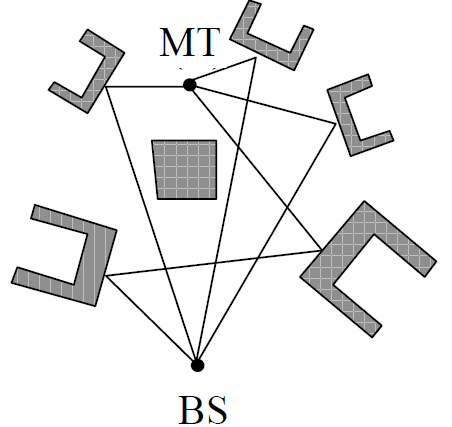
\includegraphics[scale=.5]{Figures/Propagación de señales celulares en ambientes urbanos.}
\decoRule
\caption[Propagación de señales celulares en ambientes urbanos]{Propagación de señales celulares en ambientes urbanos, [Fuente: L. Correia 2018]}
\label{fig:Propagacion}
\end{figure}

Sin embargo estas señales sufren de desvanecimiento con caídas de potencia. Este desvanecimiento depende de la posición y el ambiente del cual se propague la señal.\newline

Características de desvanecimiento:
\begin{itemize}
    \item Desvanecimiento lento:
    Depende esencialmente de la distancia, sigue una distribución Log-normal
    \item Desvanecimiento rápido:
    Es asociado al movimiento del usuario, sigue una distribución Rice
\end{itemize}

\begin{figure}[th]
\centering
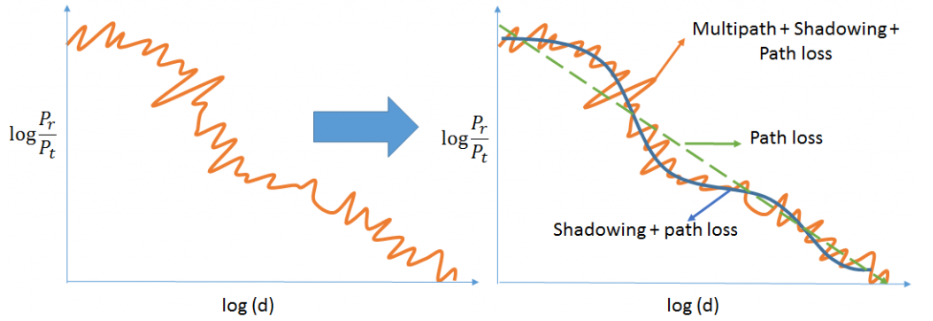
\includegraphics[scale=.8]{Figures/Ejemplo de niveles de señal con desvanecimiento lento y desvanecimiento rápido}
\decoRule
\caption[Ejemplo de niveles de señal con pérdidas por trayectoria, desvanecimiento lento y desvanecimiento rápido]{Ejemplo de niveles de señal con pérdidas por trayectoria, desvanecimiento lento y desvanecimiento rápido, [Fuente: V. Mathuranathan, 2016]}
\label{fig:Desvanecimientos}
\end{figure}

En la \textit{Figura~\ref{fig:Desvanecimientos}} se observa que al principio, la señal parece muy aleatoria. Mirando más de cerca podemos observar tres componentes principales que forman a la señal, como se muestra en la mitad derecha \parencite{Mathuranathan2016}.
\begin{enumerate}
    \item  Pérdida por trayectoria \textit{(Path loss)}
    \item  \textit{Shadowing} (Sombreado) o desvanecimiento lento
    \item  \textit{Multipath} multitrayectoria o desvanecimiento rápido.
\end{enumerate}

El desvanecimiento lento puede ser causado por eventos como el \textit{shadowing}, donde una gran obstrucción, como una colina o un gran edificio, oscurece la trayectoria de la señal principal entre el transmisor y el receptor. Se considera un parámetro a gran escala.\newline

El desvanecimiento rápido ocurre cuando la amplitud y el cambio de fase impuestos por el canal varían considerablemente durante el período de uso. Una señal que viaja en un entorno puede verse reflejada por varios objetos en el camino. Esto da lugar a varias señales reflejadas. Las señales reflejadas llegan al receptor en diferentes instantes de tiempo y con diferentes intensidades que conducen a la propagación multitrayectoria. Se considera un parámetro a pequeña escala.\newline

Cuando se habla del desvanecimiento de Rayleigh en enlaces inalambricos, en la literatura \parencite{RayleighScienceDirect} se encuentra que las componentes en cuadratura y en fase de la señal recibida son variables aleatorias Gaussianas con media cero que se distribuyen de forma independiente e idéntica (iid), siendo así, que la magnitud de la señal banda base compleja sigue una distribución de Rayleigh [Ecuación~\ref{eqn:Rayleigheqn}]. Por otra parte, la distribución de la potencia normalizada de una señal de banda base compleja recibida bajo el desvanecimiento unitario de Rayleigh es modelado por medio de una distribución exponencial unitaria [Ecuación~\ref{eqn:Exponeqn}]. \label{DesvRayleigC2} \newline 

\begin{equation}
    P_{X}(x) = {x\over\sigma_{i}^{2}}\exp\left(-{x^{2}\over 2\sigma_{i}^{2}}\right),\ x\geq 0
    \label{eqn:Rayleigheqn}
\end{equation}
Donde:
\[\sigma\to Desviación\ estándar\] 

\begin{equation}
    P_{X}(x)=\lambda e^{-\lambda x}
    \label{eqn:Exponeqn}
\end{equation}
Donde:
\[\lambda\to 1\] 

Los márgenes de desvanecimiento deben tomarse en cuenta para caracterizar la variación de las señales alrededor de un valor promedio, esto depende de:\newline

•	Características del ambiente (LoS o NLoS)\newline
•	Calidad de servicio (QoS)\newline

Para un \textit{narrowband} (banda estrecha, donde prevalece el desvanecimiento plano en lugar de un desvanecimiento selectivo de frecuencia) el desvanecimiento se caracteriza de la siguiente manera:
\begin{itemize}
    \item Desvanecimiento rápido:
    \begin{itemize}
        \item LoS: Distribución Rice (no intenso)
        \item NLoS: Distribución Rayleigh (intenso)
    \end{itemize}
    \item Desvanecimiento lento:
    \begin{itemize}
        \item Distribución Log-Normal
    \end{itemize}
    \item Ambos desvanecimiento rápido y lento:
    \begin{itemize}
        \item Distribución Susuki
    \end{itemize}
\end{itemize}

Los modelos de estimación de señal pueden ser divididos en dos categorías:
\begin{enumerate}
    \item Teóricos: Son una aproximación a la realidad, no toman en cuenta todos los factores de la propagación pero permiten cambios fáciles de los parámetros. 
    \begin{itemize}
        \item Ray Tracing
        \item Modelo Ikegami [1984]
        \item Modelo Walfish-Bertoni [1988]
    \end{itemize}
    \item Empíricos: Están basados en la observación de mediciones, conduciendo al mejor ajuste de ecuaciones. Tienen la ventaja de tomar en cuenta todos los factores que influyen en la propagación.\newline
    
    Para ambientes exteriores hay dos modelos fundamentales:
    \begin{itemize}
        \item COST 231 Okumura-Hata
        \begin{itemize}
            \item Largas distancias (>5km)
            \item Ambientes rurales, urbanos y suburbanos
            \item Alta desviacion estandar
            \item Rango de frecuencias aplicables [1.5,2.0] GHz
        \end{itemize}
        \item COST 231 Walfish-Ikegami [1999]
        \begin{itemize}
            \item Cortas distancias (<5km)
            \item Ambientes urbanos y suburbanos
            \item Rango de frecuencias aplicables [.8,2.0] GHz
        \end{itemize}
        \item COST 207 [1989]
    \end{itemize}
\end{enumerate}

\break
%----------------------------------------------------------------------------------------
%	SECTION 
%----------------------------------------------------------------------------------------

\section{ESQUEMAS DE ACCESO MÚLTIPLE AL MEDIO}
Las técnicas de acceso múltiple (MA) generalmente se pueden dividir en enfoques ortogonales y no ortogonales \parencite{Tse2004}. En MA ortogonal (OMA), los recursos de radio se dividen ortogonalmente entre dispositivos, donde las señales de diferentes dispositivos no se superponen entre sí. Las instancias de OMA son acceso múltiple por división de tiempo (TDMA), acceso múltiple por división de frecuencia (FDMA), acceso múltiple por división de frecuencia ortogonal (OFDMA), y FDMA de portadora única (SC-FDMA).\newline

\subsection{OMA}

Los enfoques OMA no tienen la capacidad de combatir la interferencia entre células \parencite{Shirvanimoghaddam2017}; por lo tanto, se requieren técnicas cuidadosas de planificación celular y gestión de interferencia para resolver este problema. \newline

Existen 4 técnicas básicas de acceso múltiple (OMA):

\begin{enumerate}
\item  Frecuencia: asignación de una portadora - FDMA (Acceso múltiple por división de frecuencia)
\item  Tiempo: asignación de un intervalo de tiempo - TDMA (Acceso múltiple por división de tiempo)
\item  Código: asignación de un código - CDMA (Acceso múltiple por división de código)
\item  Frecuencia Ortogonal: asignación de un conjunto de sub-portadoras - OFDMA (Acceso múltiple por división de frecuencia ortogonal).
\end{enumerate}

En muchos sistemas prácticos, se utiliza una mezcla o combinación de estas técnicas básicas \parencite{Correia2018}. Y también, de acuerdo a cada generación de comunicaciones móviles, el esquema de acceso al medio suele cambiar [véase Figura~\ref{fig:MAs}].\newline

\subsection{NOMA}

Igualmente, el acceso múltiple no ortogonal (NOMA) se ha convertido en un principio importante para el diseño de técnicas de acceso por radio para las redes inalámbricas de quinta generación (5G) \parencite{DIng2017}. NOMA se puede clasificar en dos categorías, el dominio de código NOMA (CD-NOMA) y el dominio de potencia NOMA (PD-NOMA). CD-NOMA utiliza diferentes códigos en el mismo recurso para lograr una ganancia de multiplexación, mientras que PD-NOMA asigna a los usuarios niveles de potencia distintos para maximizar el rendimiento. En comparación con el acceso múltiple ortogonal (OMA) que se ha aplicado ampliamente en los sistemas de comunicación inalámbrica existentes, NOMA posee el potencial de mejorar aún más la eficiencia espectral del sistema y la capacidad de conectividad.\newline

Como se mencionaba, PD-NOMA utiliza el dominio de la potencia para el acceso múltiple donde diferentes usuarios son servidos con diferentes niveles de potencia, como las señales de los diferentes usuarios se sobreponen, los receptores aprovechan la cancelación sucesiva de interferencia (SIC) para distinguir a cada una. Como varios usuarios son admitidos en la misma ranura de tiempo, frecuencia o código, la interferencia co-canal será fuerte en los sistemas NOMA \parencite{Ding2016}, por lo que no es realista el asegurar a todos los usuarios del sistema que utilicen NOMA conjuntamente, por esta razón, una alternativa es utilizar un esquema hibrido donde NOMA sea combinado con el esquema convencional ortogonal OMA. El rendimiento de este esquema hibrido es muy dependiente de como los usuarios son agrupados \parencite{Ding2016}. El agrupamiento de usuarios seleccionara a los usuarios con los que se les asignará el mismo bloque de recursos ortogonales.\newline

\begin{figure}[th]
\centering
\includegraphics[scale=1]{Figures/Cancelación Sucesiva de Interferencia (SIC)}
\decoRule
\caption[Cancelación Sucesiva de Interferencia (SIC)]{Cancelación Sucesiva de Interferencia (SIC), [Fuente: R. Kizilirmak 2017]}
\label{fig:SIC}
\end{figure}

En la \textit{Figura~\ref{fig:SIC}}, las dos señales de información indicadas con diferentes colores se superponen en el transmisor. La señal recibida en el receptor SIC incluye todas estas tres señales. La primera señal que SIC decodifica es la más fuerte, mientras que la otra es tratada como ruido. La primera señal decodificada se resta de la señal recibida y si la decodificación es perfecta, la forma de onda con la otra señal se obtiene con precisión. SIC itera el proceso hasta que encuentra la señal deseada \parencite{Kizilirmak2016}.\newline

\begin{figure}[th]
\centering
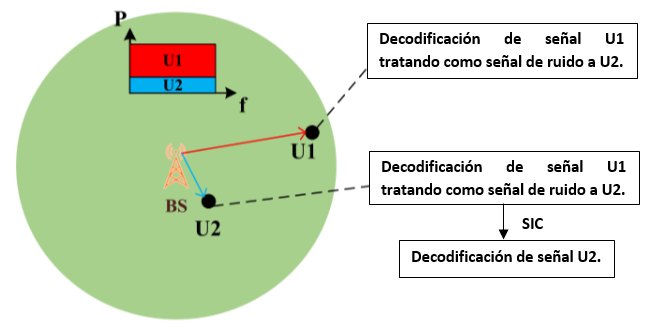
\includegraphics[scale=1]{Figures/Ejemplo del esquema NOMA en un enlace de bajada con dos usuarios y una sub-portadora}
\decoRule
\caption[Ejemplo del esquema NOMA en un enlace de bajada con dos usuarios y una sub-portadora.]{Ejemplo del esquema NOMA en un enlace de bajada con dos usuarios y una sub-portadora, [Fuente: Ding 2017]}
\label{fig:NOMADL}
\end{figure}

Como se muestra en la \textit{Figura~\ref{fig:NOMADL}}, la idea clave del NOMA en el dominio de potencia es asignar más potencia al usuario con condiciones de canal más pobres. El usuario 1 decodifica su propio mensaje directamente tratando el mensaje del usuario 2 como ruido y por otro lado, el usuario 2 realiza SIC, es decir, primero decodifica el mensaje del usuario 1 y luego elimina este mensaje de su observación antes de decodificar su propio mensaje.

Suponga que el usuario 1 es un dispositivo IoT que requiere solo una baja velocidad de datos, y el usuario 2 es un usuario que exige una alta velocidad de datos. Cuando se utiliza OFDMA, que es un ejemplo típico de OMA, cada usuario se asigna a la sub-portadora. En este ejemplo, la eficiencia espectral de OMA es pobre ya que el dispositivo IoT tiene más ancho de banda de lo que realmente necesita, mientras que al usuario de banda ancha no se le asigna suficiente ancho de banda. Por otro lado, el uso de NOMA fomenta el intercambio de espectro, es decir, el usuario de banda ancha también puede tener acceso a la sub-portadora ocupada por el dispositivo IoT, en la F\textit{igura 24} se puede observar gráficamente la asignación del espectro en los dos esquemas.

\begin{figure}[th]
\centering
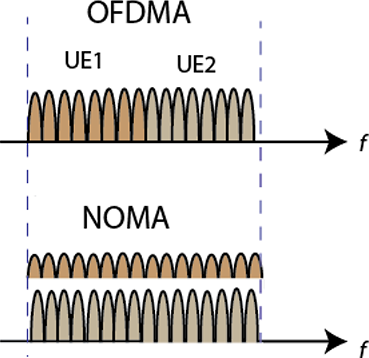
\includegraphics[scale=1]{Figures/Ejemplo del espectro compartido para OFDMA y NOMA con dos usuarios}
\decoRule
\caption[Ejemplo del espectro compartido para OFDMA y NOMA con dos usuarios.]{Ejemplo del espectro compartido para OFDMA y NOMA con dos usuarios, [Fuente: R. Kizilirmak 2017]}
\label{fig:OFDMANOMA}
\end{figure}

Dada la madurez técnica de OFDMA, es muy probable que este tipo de OMA se incorpore a las redes 5G \parencite{DIng2017} y la forma en que múltiples sub-portadoras OFDMA se pueden combinar de manera eficiente con NOMA ha recibido mucha atención.

Acerca del uso de arreglos múltiples de antenas (MIMO) para NOMA, han sido tema de mucho interés que han estado estudiandose para poder alcanzar un rendimiento óptimo del sistema, el ordenamiento de usuarios en escenarios de MIMO-NOMA es una tarea difícil \parencite{DIng2017}. En el caso de SISO, los canales de los usuarios son escalados, por lo que es sencillo ordenar a los usuarios de acuerdo con las condiciones de su canal. Sin embargo, cuando los nodos están equipados con antenas múltiples, los canales de los usuarios están en forma de vectores o matrices, lo que significa que ordenar a los usuarios de acuerdo con las condiciones de sus canales como en el caso SISO se vuelve difícil. 

\subsection{Interfaz de Radio}
Los canales de transmisión dirigidos desde la BS a MT son referidos como canal \textit{downlink} y los dirigidos desde el MT a la BS como canales \textit{uplink}, estos canales juntos se identifican como canales ``dúplex'. La transmisión bidireccional de la información en sistemas dúplex puede dividirse en \parencite{Correia2018}:

\begin{enumerate}
\item  Frecuencia: Donde los canales UL y DL ocupan diferentes bandas de frecuencia - FDD (\textit{Frequency Division Multiplexing}).
\item  Tiempo: Donde los canales UL y DL ocupan diferentes ventanas de tiempo- TDD (\textit{Time Division Multiplexing}).
\end{enumerate}

FDD se caracteriza por: 
\begin{itemize}
\item  Cuando es utilizada una división ``dúplex'' de frecuencia FDD estos canales son transmitidos en diferentes frecuencias
\item  Permitir transmisión simultánea en ambos caminos
\item  Requieren filtros con un buen rechazo en la banda adyacente
\item  Requieren en general el uso de filtros dúplex
\end{itemize}

TDD se caracteriza por: 
\begin{itemize}
\item  Cuando se usa una división ``dúplex'' de tiempo TDD los canales son transmitidos en la misma frecuencia pero utilizando diferentes ranuras de tiempo.
\item  Permitir transmisión secuencial en ambos caminos
\item  Requiere sincronización
\item  No requieren uso de filtros dúplex
\end{itemize}

El uso de una técnica de división dúplex puede depender de la técnica de acceso múltiple utilizada para el sistema.

%----------------------------------------------------------------------------------------
%	SECTION 
%----------------------------------------------------------------------------------------

\section{GENERACIONES PASADAS DE LOS SISTEMAS DE COMUNICACIÓN MÓVIL}

La generación 1G fue la primera generación de tecnología celular inalámbrica. 1G se introdujo en la década de 1980. Las señales de radio utilizadas por la red 1G fueron analógicas y proporcionaba comunicación solo por voz, alcanzaba una velocidad de 2.4 Kbps. La técnica de acceso múltiple utilizada en 1G es el acceso múltiple por división de frecuencia (FDMA) [véase Figura~\ref{fig:MAs}]\parencite{Nair2018}. Esta generación utiliza el método de conmutación de circuitos para la transmisión de datos. \newline

Las redes celulares 2G de segunda generación fueron lanzadas comercialmente en el estándar GSM en Finlandia 1991 \parencite{Nair2018}. 2G utilizó el método de conmutación de paquetes para la transmisión de datos y habilitó el cifrado digital de la conversación por teléfono, además proporcionaron servicios multimedia como SMS (Servicios de mensajes cortos) MMS (Servicios de mensajes multimedia) y las velocidades de descarga y carga fueron de hasta 236 Kbps. Se utilizó el acceso múltiple por división de tiempo (TDMA), como el número de usuarios aumentó con el tiempo, TDMA se volvió obsoleto por causar una velocidad más baja para cada usuario.\newline

3G (conocida también como UMTS) fue la tercera generación de tecnología inalámbrica de telecomunicaciones móviles y utilizó el acceso múltiple por división de código de secuencia directa (DS-CDMA) \parencite{Nair2018}. Las redes 3G ofrecieron velocidades de 3.1 megabits por segundo (Mbps) o más y se instalaron por primera vez en 1998. La aplicación del concepto 3G se encuentra en telefonía inalámbrica, acceso a Internet móvil, acceso a Internet inalámbrico, llamadas de conferencia y TV portátil.\newline

\begin{figure}[th]
\centering
\includegraphics[scale=.6]{Figures/Diferentes tipos de acceso múltiple}
\decoRule
\caption[Diferentes tipos de acceso múltiple al medio ocupados en generaciones anteriores (1G, 2G y 3G)]{Diferentes tipos de acceso múltiple al medio ocupados en generaciones anteriores (1G, 2G y 3G), [Fuente: https://www.itu.int/osg/spuold/ni/3g/technology/index.html]}
\label{fig:MAs}
\end{figure}

4G (conocida también como LTE) es el término utilizado para describir la cuarta generación de servicio celular inalámbrico y es el estándar actual del servicio celular. Es hasta 10 veces más rápido que los servicios 3G. Sprint fue el primer operador en ofrecer velocidades 4G en los EE. UU a partir de 2009. Las redes 4G pueden ofrecer velocidades de descarga entre 5 y 12 Mbps y velocidades de carga entre 2 y 5 Mbps, lo que finalmente da una velocidad máxima de 50Mbps. El sistema de comunicación celular 4G utiliza una versión avanzada del esquema FDMA, es decir, OFDMA (acceso múltiple por división de frecuencia ortogonal) \parencite{Nair2018}.\newline

%----------------------------------------------------------------------------------------
%	SECTION 
%----------------------------------------------------------------------------------------

\section{SISTEMAS DE COMUNICACIONES MÓVILES DE QUINTA GENERACIÓN (5G)}

La NGMN define su visión de una red 5G de la siguiente manera: "5G es un ecosistema de extremo a extremo para permitir una sociedad totalmente móvil y conectada."\newline

La anteriores generaciones de comunicaciones móviles (1G,{\dots},4G) han sido transformadoras en el sentido que fueron motivadas para mejorar los tradicionales KPIs de la red, sin embargo la nueva generación de comunicaciones móviles (5G) aparte de ser transformadora viene a ser disruptiva ante las generaciones anteriores ya que propone nuevas técnicas, modelos y KPIs que habilitarán una gama amplia de servicios con alta fiabilidad, ayudando a conformar toda una red heterogénea global móvil interconectada con altos índices de rendimiento.\newline

La investigación sobre los casos de uso de una red 5G y sus requisitos técnicos han sido realizadas por la ITU-R, el 3GPP y la NGMN:

\begin{figure}[th]
\centering
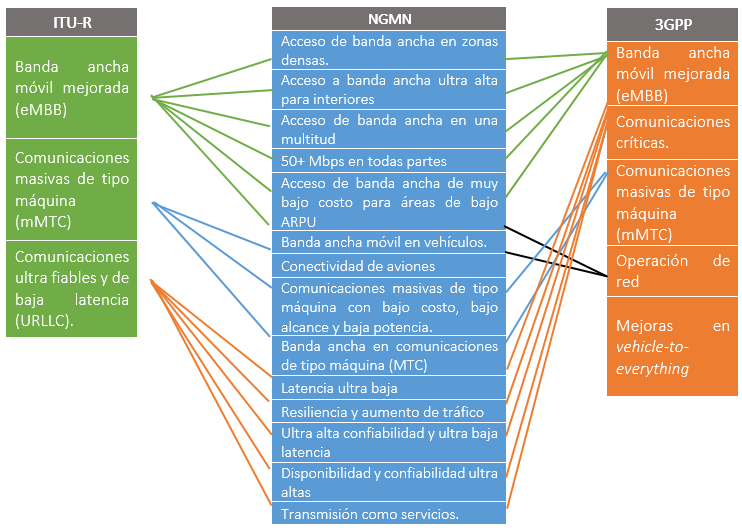
\includegraphics[scale=1]{Figures/Comparación de diversos escenarios de uso de la tecnología 5G}
\decoRule
\caption[Comparación de diversos escenarios de uso de la tecnología 5G por la UIT-R, el 3GPP y la NGMN]{Comparación de diversos escenarios de uso de la tecnología 5G por la UIT-R, el 3GPP y la NGMN}
\label{fig:5g}
\end{figure}

5G admitirá una gran variedad de casos de uso que están surgiendo ahora o surgirán en el futuro. Los diversos casos de uso tienen características y requisitos variables. Es útil agrupar innumerables casos de uso emergentes en varias familias de casos de uso. \newline

La \textit{Figura~\ref{fig:5g}} muestra las ocho familias de casos de uso por la NGMN con un ejemplo de caso de uso para cada familia, y sus correspondientes ejemplos de casos de uso con la 3GPP y la ITU-R.\newline

En términos generales, ITU-R ha concluido tres casos de uso para abordar la gran variedad de requisitos y características \parencite{5gMobileComms}:

\begin{enumerate}
    \item \textbf{Banda ancha móvil mejorada} \textbf{(eMBB)}: la banda ancha móvil aborda casos de uso centrados en el hombre para acceder a contenido multimedia, servicios y datos. La demanda de banda ancha móvil seguirá aumentando, lo que dará lugar a una banda ancha móvil mejorada. El escenario mejorado de uso de banda ancha móvil vendrá con nuevas áreas de aplicación y requisitos, además de las aplicaciones de banda ancha móvil existentes para un mejor rendimiento y una experiencia de usuario cada vez más perfecta.
    \item \textbf{Comunicaciones ultra fiables y de baja latencia (URLLC)}: este caso de uso tiene requisitos estrictos para capacidades tales como rendimiento, latencia y disponibilidad. Algunos ejemplos incluyen el control inalámbrico de la fabricación industrial o los procesos de producción, cirugía médica remota, automatización de la distribución en una red inteligente, seguridad en el transporte, manejo autónomo de automóviles, etc.
    \item \textbf{Comunicaciones masivas de tipo máquina (mMTC)}: este caso de uso se caracteriza por un gran número de dispositivos conectados que transmiten un volumen relativamente bajo de datos no sensibles al retardo. Los dispositivos deben ser de bajo costo y tener una batería de larga duración.
\end{enumerate}

%----------------------------------------------------------------------------------------
%	SECTION 
%----------------------------------------------------------------------------------------

\section{INTERNET DE LAS COSAS (IoT)}


El internet de las cosas (IoT) es una emergente y prometedora tecnología que habilitará la interconexión del mundo global a través de la conexión de objetos físicos (comúnmente dispositivos de bajo consumo) mediante el uso del internet \parencite{5GSurveyAkpaku}. Una de las características más importantes de esta tecnología es que ocupa la comunicación máquina a máquina (M2M) con el fin de que los dispositivos se conecten y comuniquen entre sí sin alguna intervención humana.\newline

Para habilitar esta tecnología se requiere el soporte para conexiones masivas, es decir, admitir la gran cantidad de sensores en una sola celda. Debido a que la mayoría de estos sensores deben operar durante varios años, la eficiencia energética en las transmisiones inalámbricas es un requisito importante. Además, se debe reducir el costo de implementación de tales sensores \parencite{IoT5GWire}.

\break
%----------------------------------------------------------------------------------------
%	SECTION 
%----------------------------------------------------------------------------------------

\section{MODELADO DEL TRÁFICO EN TELECOMUNICACIONES}

Conceptos básicos:
\begin{enumerate}
\item  \underbar{Tráfico}: Es el acumulado de peticiones de servicio de todos los usuarios atendidos por la red o por una parte de ella.
\item  \underbar{Recurso o servidor}: medio físico, usualmente sólo es capaz de atender un solo servicio.
\item  \underbar{Sistema de colas}: conjunto de servidores de uso compartido.
\end{enumerate}

\subsection{Caracterización del Tráfico}
Para caracterizar el tráfico se deben definir previamente los siguientes conceptos:
\begin{enumerate}
\item  \underbar{Volumen de Tráfico Cursado}. Suma de la duración de todos los servicios atendidos por el sistema.
\item  \underbar{Intensidad de Tráfico Cursado u Ocupación promedio de recursos (a')}. Número promedio de servicios atendidos simultáneamente. Se puede obtener mediante dividir el volumen de tráfico cursado entre el tiempo que tomó cursar dicho volumen. También se puede interpretar como el número promedio de servidores ocupados.
\item  \underbar{Intensidad de Tráfico Ofrecido (a).} Número promedio de servicios atendidos simultáneamente, si todas las peticiones fueran atendidas.
\end{enumerate}

Suponiendo un sistema que es capaz de atender todas las peticiones de servicio y al que arriban $\lambda$ peticiones/segundo. Esto implica que en un intervalo T segundos se recibirían $\lambda$$\cdot$T peticiones de servicio. Si la duración promedio de estos servicios es $\mu$ segundos, entonces el volumen de tráfico ofrecido (y en este caso también cursado) es $\lambda$$\cdot$$\mu$$\cdot$T y la intensidad de tráfico ofrecido se reduce a:
\begin{equation}
    a=\lambda\cdot\mu
    \label{eqn:a}
\end{equation}

Para un sistema que atiende todas las peticiones el tráfico cursado y el ofrecido son iguales, sin embargo, cuando se analizan sistemas que no cumplan esta característica, a se vuelve un valor hipotético (la intensidad de tráfico cursado, si todas las peticiones se atendieran), sin embargo, seguirá describiendo la intensidad del tráfico que se ofrece. Es importante mencionar que el desempeño de un sistema (en términos de algún parámetro de calidad de servicio) no va a depender del valor de $\lambda$ o de $\mu$ por sí solos, sino del producto de ellos. Por ejemplo, un sistema se puede saturar tanto por una alta tasa de arribos como por una gran duración del tiempo de servicio.\newline

\subsection{Modelado de tiempos entre llegadas}

Sean $X1, X2, X3, ... Xi$ variables aleatorias tales que:
\begin{itemize}
    \item $X1$ = el intervalo de tiempo entre el inicio del proceso y el primer evento, es decir, la primera llegada,
    \item $X2$ = el tiempo entre llegadas entre la primera y la segunda llegada,
    \item $X3$ = el tiempo entre llegadas entre la segunda y la tercera llegada , y así sucesivamente.
\end{itemize}
La distribución de la variable aleatoria $Xk$ que representa el tiempo entre llegadas entre la llegada $(k-1) th$ y $(k) th$ es \parencite{PoissonMedium}:
\begin{equation}
    X_{k}=Exponential(\lambda)
    \label{eqn:expon}
\end{equation}
La Función Densidad de Probabilidad (PDF) de la variable aleatoria $X_{k}$ es la siguiente:
\begin{equation}
    P_{X}(t)=\lambda e^{-\lambda t}
    \label{eqn:pdfexpon}
\end{equation}
Y describe la PDF de tiempos entre llegadas en un proceso de Poisson.\newline

Hasta este punto el tráfico sólo se ha caracterizado en término de dos valores promedio: la tasa de arribos ($\lambda$) y la duración promedio de los servicios ($\mu$). Estos parámetros representan información parcial de dos variables aleatorias, el tiempo entre arribos (TEA) y el tiempo duración de servicio (TDS). Estos tiempos por su carácter aleatorio en muchos análisis se modelan como variables aleatorias. El tipo de comportamiento aleatorio en las tasas se establece al de una distribución exponencial negativa \parencite{Carter1990}. La tasa de arribos corresponde una distribución como sigue:

\begin{equation}
f(y)=\lambda e^{-\lambda y}\cdot u(y)
\label{eqn:lambda}
\end{equation}

La duración promedio de servicios corresponde a:
\begin{equation}
f(y)=\frac{1}{\mu } e^{-\frac{1}{\mu} y} \cdot u(y)
\label{eqn:mu}
\end{equation} 

Es necesario establecer fórmulas que relacionen a la cantidad de recursos y el tráfico ofrecido con los parámetros de calidad de servicio, se requiere como paso intermedio determinar la probabilidad de que el sistema se encuentre en determinado estado.\newline

Se considera que el sistema está en estado j, si la suma de los servicios que están siendo atendidos más los servicios en espera es j.\newline

Una técnica que simplifica significativamente el cálculo de las probabilidades de estado es el uso de cadenas de Markov, sin embargo, la solución mediante este método implica el análisis del sistema exclusivamente en el dominio de las probabilidades, por lo que las probabilidades de estado no tienen dependencia del tiempo. Esta independencia del tiempo se consigue sólo si:

\begin{enumerate}
\item  El sistema se analiza en estado estable, es decir, si el sistema ha estado operando por un intervalo de tiempo lo suficientemente grande, de modo que ya no depende de las condiciones iniciales.
\item  Si la probabilidad de que el sistema cambie de estado no depende de cuánto tiempo haya permanecido en el estado actual.
\end{enumerate}

 La segunda condición sólo se puede cumplir si las distribuciones del TEA y del TDS son exponenciales negativas \parencite{Carter1990}.\newline

 Si el número de servidores que posee un sistema es menor a la cantidad de fuentes que generan el tráfico, y se entiende como fuentes de tráfico a los posibles usuarios, resulta imposible atender a todas las peticiones de servicio de forma instantánea. Básicamente se puede proceder de 2 formas con aquellas llamadas que hallen al sistema saturado:
\begin{enumerate}
\item  Negarles el servicio. Se tiene un sistema con bloqueo o con pérdidas.
\item  Mantenerlas en espera y asignarles servidores cuando sean liberados. Se tiene un sistema con retardo.
\end{enumerate}

 En el modelado de los sistemas con bloqueo también se debe tomar en cuenta que sucede con las llamadas que no son atendidas y dependiendo de la naturaleza del servicio analizado se puede considerar que las llamadas bloqueadas regresan al sistema en forma de reintentos o bien son eliminadas en forma definitiva.\newline

 Otra consideración de suma importancia en el sistema de colas es tomar en cuenta que tan grande es la cantidad de posibles fuentes de tráfico en comparación con la cantidad de recursos; cuando la cantidad de fuentes es muy grande se puede aproximar con infinito y los análisis se simplifican considerablemente.\newline

 También es importante mencionar que hay sistemas en los que las peticiones pueden experimentar bloqueo o retardo. Además de las consideraciones previas: la distribución del TEA y del TDS, la cantidad de recursos y el tamaño de la cola de espera son parámetros que influyen en el desempeño de un sistema.

 \subsection{Notación Kendall}

 Para describir a un sistema mediante estos parámetros se puede usar la notación de Kendall, la cual se expresa de la forma:
$c1/ c2/ s/ K$

 Donde:
\begin{enumerate}
    \item  \textbf{c1} representa la distribución del TEA y pueden asignársele las letras M (arribos Markovianos, es decir distribución exponencial negativa) o G (General, es decir cualquier otra distribución).
    \item  \textbf{c2} es la distribución del TDS y puede ser M (exponencial negativa), D (Determinístico, es decir el TDS es constante) o G (general).
    \item  \textbf{s} es el número de servidores.
    \item  \textbf{K} es la longitud de la cola de espera.
\end{enumerate}

 Se refiere como $\lambda$ a la tasa de arribos generada por todas las fuentes de tráfico y se denotó anteriormente $\mu$ a la duración promedio de un servicio. El inverso de dicho tiempo se considera la tasa a la que finaliza un servicio en curso. En caso de que existan j servicios en curso la tasa a la que finalizan las llamadas es j/$\mu$. Esta fórmula concuerda con el hecho de que a medida que hay más servicios en curso, menos tiempo se tiene que esperar a que alguno de ellas finalice, es decir, la tasa de finalización se incrementa.

 La probabilidad de bloqueo está dada por:
\begin{equation}
    P_{j}=\frac{\frac{(\lambda\mu)^{j}}{j!}}{\sum_{k=0}^{s}\frac{(\lambda\mu)^{k}}{k!}}
    \label{eqn:Pb}
\end{equation} 
De todas las probabilidades de estado, Ps tiene particular importancia, ya que representa la probabilidad de que el sistema esté saturado, en otras palabras, la probabilidad de bloqueo:
\begin{equation}
    P_{s}=\frac{\frac{a^{s}}{s!}}{\sum_{k=0}^{s}\frac{a^(k)}{k!}}
    \label{eqn:Ps}
\end{equation} 

La Ecuación~\ref{eqn:Ps} fue desarrollada originalmente por el danés A. K. Erlang, por lo que es comúnmente conocida como fórmula de \textbf{Erlang-B}.\newline

Notese que en la Ecuación~\ref{eqn:Pb} el producto $\lambda \mu$ se puede sustituir por a, el tráfico ofrecido, y con esto se corrobora que la calidad del servicio (en este caso la probabilidad de bloqueo) no depende de $\lambda$ o de $\mu$ por si solos, sino de su producto.\newline

%----------------------------------------------------------------------------------------
%	SECTION 
%----------------------------------------------------------------------------------------

\section{SIMULACIÓNES A NIVEL DE SISTEMA}

Debido a las complicadas estructuras de los sistemas de comunicación celular móvil, no podemos describirlos completamente a través de un modelo matemático simple y abstracto. Por lo tanto, siempre recurrimos a la simulación para evaluar su rendimiento. La simulación a nivel de sistema se ha utilizado ampliamente para evaluar el rendimiento integral de diferentes sistemas celulares móviles \parencite{Chen2011}. Los programas de computadora se utilizan para simular los mecanismos operativos de los sistemas móviles de comunicación celular, los tráficos cargados, etc. El rendimiento de estos sistemas se puede reflejar en última instancia por los resultados obtenidos de los programas de simulación.\newline

\begin{figure}[th]
\centering
\includegraphics[scale=.6]{Figures/El diseño usual de una red celular en simulaciones a nivel de sistema}
\decoRule
\caption[El diseño usual de una red celular en simulaciones a nivel de sistema]{El diseño usual de una red celular en simulaciones a nivel de sistema}
\label{fig:sim_sistema}
\end{figure}

El escenario para la simulación a nivel de sistema generalmente consiste en una red con múltiples BS y MS [\textit{véase Figura~\ref{fig:sim_sistema}}]. A diferencia de la simulación a nivel de enlace, la simulación a nivel de sistema se centra en las métricas de rendimiento de la capa de aplicación expresadas por el rendimiento del sistema, la imparcialidad del usuario, la calidad de servicio percibida por el usuario (QoS), el retraso de la transferencia o la tasa de éxito, etc.

%----------------------------------------------------------------------------------------
%	SECTION 
%----------------------------------------------------------------------------------------

\section{SIMULACIONES ORIENTADAS A EVENTOS DISCRETOS}


Una simulación es casi siempre la imitación de algún proceso o sistema que toma o podría tomar lugar en el mundo real, implementada utilizando un paradigma de programación y ejecutada por computadoras. Para realizarse esta, debe tenerse en cuenta un previo estudio del sistema real o de algún modelo o modelos existentes, junto con un análisis detallado de las variables presentes, además es necesario hacer distintas suposiciones al estar el estándar aún en desarrollo. Todo esto para permitir una simulación que simplifique el sistema, pero aun siendo capaz de generar resultados que puedan ayudar a su caracterización y a ser dimensionado. \newline

En \parencite{Banks2005} se describe a un sistema discreto como: \textit{``[{\dots}] aquel en el cual las variables de estado cambian únicamente en un número discreto de instantes en el tiempo''.} Por lo que la simulación de eventos discretos es la implementación en hardware de un sistema en el que sus variables de estado cambian de tal forma con el arribo de eventos, los cuales se tratan de ocurrencias que se presentan de forma instantánea y cuentan con un nacimiento y una muerte.\newline

En cuanto a un evento o proceso estocástico, tenemos la siguiente definición \parencite{Correia2018}:\newline

\textit{Definición: Un proceso estocástico es una colección de variables aleatorias $X_{t}:t\in T$ parametrizada por un conjunto T, llamado espacio parametral, en donde las variables toman valores en un conjunto S llamado espacio de estados.}\newline

\textit{En los casos más sencillos se toma como espacio perimetral al conjunto discreto}\newline

\textit{T = [0, 1, 2,...] y estos números se interpretan como tiempos. En este caso se dice que el proceso es a tiempo discreto, y en general este tipo de procesos se denotara  por [Xn: n = 0, 1,. . .]} 

\subsection{Lenguajes de Programación para simulaciones orientadas a eventos discretos(DES)}

Considerando solamente los lenguajes que sean de código abierto, tenemos a \textit{JAVA (DESMO-J y Ptolomeo I), Python (Simpy) y C++ (SystemC y PowerDEVS)} como los lenguajes más conocidos y de entre estos sobresalen \textit{Simpy }(P\textit{ython}) y \textit{SystemC }(\textit{C++) }como los que han tenido más soporte y actualización (2018), lo cual será un factor importante al elegir el lenguaje.\newline

Simpy es una librería basada en procesos, se pueden definir diferentes entornos, todos los procesos interactúan mediante eventos con el mismo entorno y entre ellos. Durante su estancia, los procesos crean eventos y producen nuevos eventos para esperar a que se activen. Cuando un proceso produce un evento, el proceso se suspende, SimPy reanuda el proceso, cuando ocurre el evento. Varios procesos pueden esperar el mismo evento, SimPy los reanuda en el mismo orden en que dieron lugar a ese evento \parencite{Simpy}. Además proporciona varios tipos de recursos compartidos para modelar puntos de congestión de capacidad limitada (p. ej. servidores).\newline

La documentación de SimPy contiene tutoriales, guías detalladas y una gran cantidad de ejemplos \parencite{Simpy}. SimPy se lanza como software de código abierto bajo la licencia del MIT. La primera versión fue lanzada en diciembre de 2002 y hoy en día su última versión estable es la 3.0.11 / 16 de noviembre de 2018.\newline

Python es un lenguaje de programación dinámico de alto nivel, interpretado y de propósito general que se enfoca en la legibilidad del código. La sintaxis en Python ayuda a los programadores a codificar en menos pasos en comparación con Java o C ++ \parencite{PythonVentajas}. Python es ampliamente utilizado en organizaciones más grandes debido a sus múltiples paradigmas de programación. Usualmente involucran programación funcional imperativa y orientada a objetos. \newline

\subsection{Python}

Ventajas o beneficios de Python \parencite{PythonVentajas}:
\begin{enumerate}
\item  Característica de integración
\item  Productividad mejorada del programador
\item  Amplias librerías de soporte:
\end{enumerate}

Scipy es una librería de Python utilizada para la informática científica y la informática técnica. \newline

NumPy es una librería de Python utilizada para la informática científica que, aparte de sus usos científicos, puede utilizarse como un contenedor multidimensional para datos genéricos.\newline

Matplotlib es una librería para la generación de gráficos a partir de datos contenidos en listas o arrays en el lenguaje de programación Python y su extensión matemática NumPy. Proporciona una API, pylab, diseñada para recordar a la de MATLAB.\newline

Desventajas o Limitaciones de Python:
\begin{enumerate}
\item  Lenguaje interpretado: se ralentiza en velocidad: Python se ejecuta con la ayuda de un intérprete en lugar del compilador, lo que hace que se ralentice porque la compilación y la ejecución ayudan a que funcione normalmente.
\end{enumerate}

El mecanismo que degrada el desempeño de CPython es la ejecución de bytecode por varios hilos a la vez, conocido como \textit{Global Interpreter Lock} o GIL, es un mecanismo utilizado en intérpretes de lenguaje de computadora para sincronizar la ejecución de subprocesos para que solo un subproceso nativo pueda ejecutarse a la vez. Un intérprete que usa GIL siempre permite que se ejecute exactamente un subproceso a la vez, incluso si se ejecuta en un procesador multinúcleo.

\subsection{Multiprocesamiento}
Afortunadamente, existen métodos para evitar este comportamientto del interpretador, haciendo que se usen todos los nucleos del PC con ayuda de la librería \textit{multiprocessing} \parencite{Multiprocessing}.\newline
\begin{figure}[th]
    \centering
    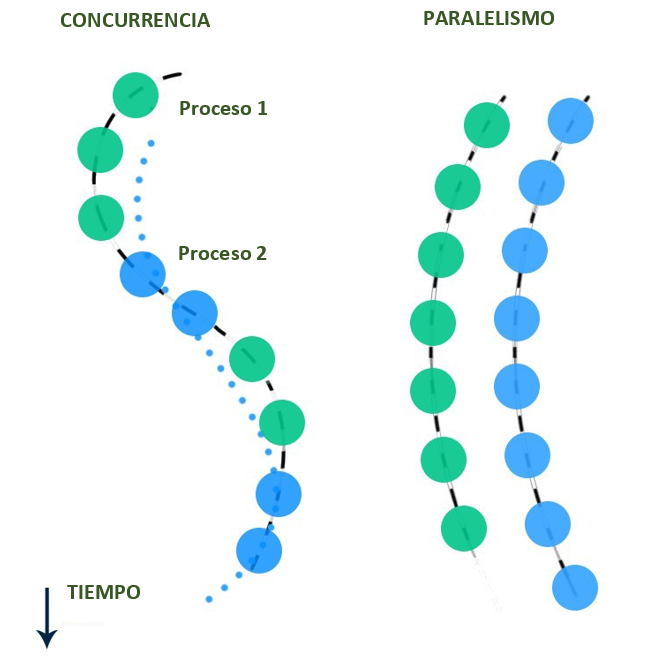
\includegraphics[scale=.35]{Figures/Multiprocesamiento}
    \decoRule
    \caption[Concurrencia Vs Paralelismo]{Concurrencia  Vs Paralelismo}
    \label{fig:multiprocessing}
\end{figure}

El módulo de multiprocessing permite al programador aprovechar al máximo múltiples procesadores en paralelo. Se ejecuta tanto en Unix como en Windows, no confundir con concurrencia (esta hace uso de múltiples hilos) [véase Figura~\ref{fig:multiprocessing}].
\hfill 

\break






%----------------------------------------------------------------------------------------
%	SECTION 
%----------------------------------------------------------------------------------------

\section{ORGANISMOS INTERNACIONALES DE ESTANDARIZACIÓN}

Para la creación de estándares de las redes de nueva generación, existen más que en otras ocasiones, organizaciones desarrolladoras de estándares de telecomunicaciones (TSDOs) \parencite{3GPP2019}, lo que significa que hay muchas partes que debieran moverse en armonía. Estas organizaciones comparten entre sí: sus recomendaciones, artículos, especificaciones, estándares, presentaciones, visiones y demás. \newline

Unos de los TSDO más importantes que han contribuido a definir el funcionamiento de redes móviles como por ejemplo UMTS, LTE, NB-IoT entre otros, es el Proyecto de Asociación de 3ra Generación (3GPP), el cual unifica a siete organizaciones internacionales de desarrollo de estándares de telecomunicaciones (ARIB, ATIS, CCSA, ETSI, TSDSI, TTA, TTC), conocidas en conjunto como "Socios Organizacionales". 3GPP proporciona a sus miembros un entorno estable para producir los Informes y Especificaciones que definen las tecnologías 3GPP \parencite{3GPP2019}. El proyecto cubre tecnologías de telecomunicaciones celulares, incluyendo acceso de radio, red central y capacidades de servicio, que proporcionan una descripción completa del sistema para comunicaciones móviles. \newline


\begin{figure}[th]
\centering
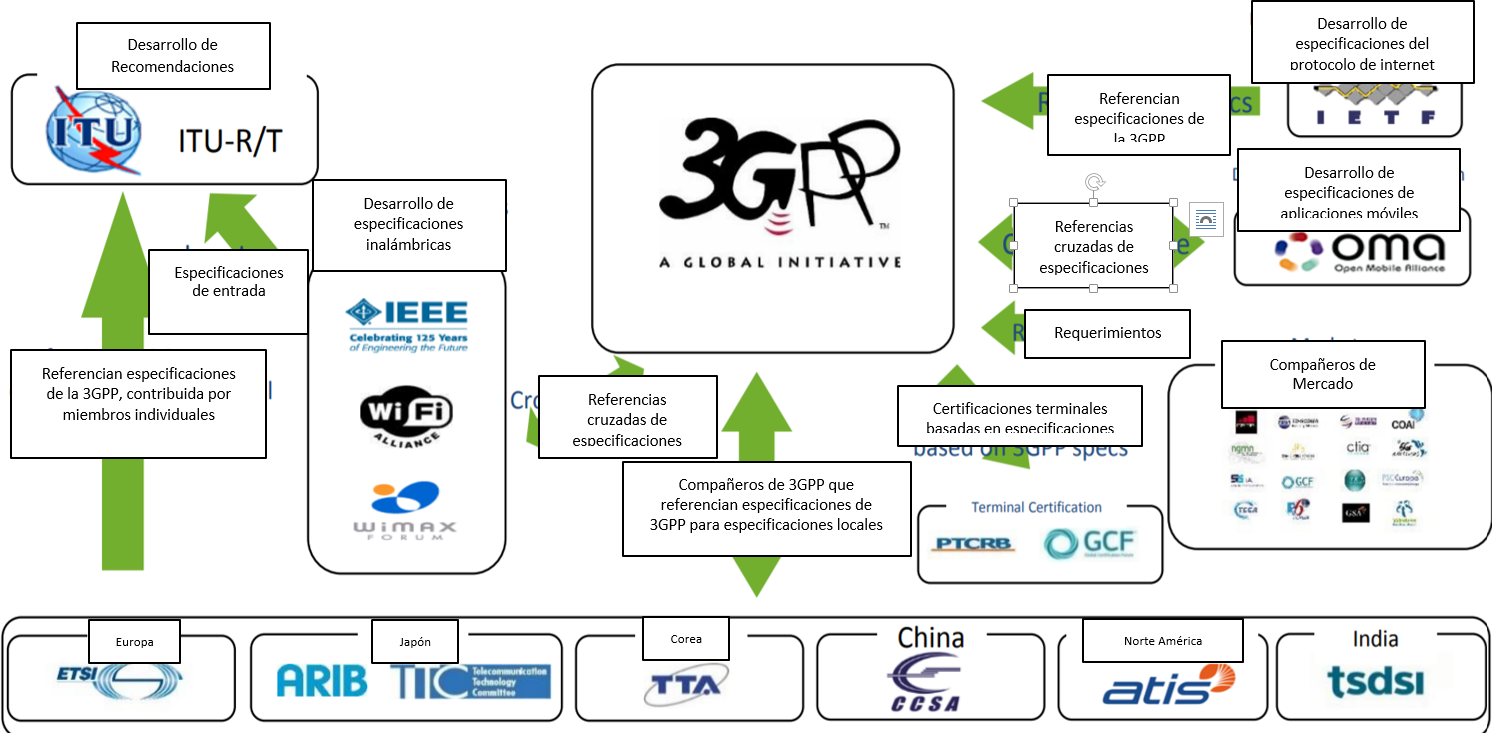
\includegraphics[scale=.5]{Figures/Socios Internacionales con los que colabora la 3GPP}
\decoRule
\caption[Socios Internacionales con los que colabora la 3GPP]{Socios Internacionales con los que colabora la 3GPP, [Fuente: https://www.3gpp.org/about-3gpp/partners]}
\label{fig:socios}
\end{figure}

Además, los socios organizacionales de 3GPP pueden invitar a un socio de representación del mercado a participar en 3GPP, con el fin de ofrecer asesoramiento de mercado a 3GPP y traer a 3GPP una visión consensuada de los requisitos del mercado [\textit{véase Figura~\ref{fig:socios}}].\newline

Los tres grupos de especificaciones técnicas (TSG, \textit{Technical Specifications Group}) de 3GPP,  quienes cada determinado tiempo liberan \textit{releases} (lanzamientos) en los cuales especifican estándares \parencite{3GPP2019}, son:

\begin{enumerate}
\item  Redes de acceso por radio (RAN).
\item  Servicios y aspectos de sistemas (SA).
\item  Red central y terminales (CT).
\end{enumerate}